% Template for PLoS
% Version 3.1 February 2015
%
% To compile to pdf, run:
% latex plos.template
% bibtex plos.template
% latex plos.template
% latex plos.template
% dvipdf plos.template
%
% % % % % % % % % % % % % % % % % % % % % %
%
% -- IMPORTANT NOTE
%
% This template contains comments intended 
% to minimize problems and delays during our production 
% process. Please follow the template instructions
% whenever possible.
%
% % % % % % % % % % % % % % % % % % % % % % % 
%
% Once your paper is accepted for publication, 
% PLEASE REMOVE ALL TRACKED CHANGES in this file and leave only
% the final text of your manuscript.
%
% There are no restrictions on package use within the LaTeX files except that 
% no packages listed in the template may be deleted.
%
% Please do not include colors or graphics in the text.
%
% Please do not create a heading level below \subsection. For 3rd level headings, use \paragraph{}.
%
% % % % % % % % % % % % % % % % % % % % % % %
%
% -- FIGURES AND TABLES
%
% Please include tables/figure captions directly after the paragraph where they are first cited in the text.
%
% DO NOT INCLUDE GRAPHICS IN YOUR MANUSCRIPT
% - Figures should be uploaded separately from your manuscript file. 
% - Figures generated using LaTeX should be extracted and removed from the PDF before submission. 
% - Figures containing multiple panels/subfigures must be combined into one image file before submission.
% For figure citations, please use "Fig." instead of "Figure".
% See http://www.plosone.org/static/figureGuidelines for PLOS figure guidelines.
%
% Tables should be cell-based and may not contain:
% - tabs/spacing/line breaks within cells to alter layout or alignment
% - vertically-merged cells (no tabular environments within tabular environments, do not use \multirow)
% - colors, shading, or graphic objects
% See http://www.plosone.org/static/figureGuidelines#tables for table guidelines.
%
% For tables that exceed the width of the text column, use the adjustwidth environment as illustrated in the example table in text below.
%
% % % % % % % % % % % % % % % % % % % % % % % %
%
% -- EQUATIONS, MATH SYMBOLS, SUBSCRIPTS, AND SUPERSCRIPTS
%
% IMPORTANT
% Below are a few tips to help format your equations and other special characters according to our specifications. For more tips to help reduce the possibility of formatting errors during conversion, please see our LaTeX guidelines at http://www.plosone.org/static/latexGuidelines
%
% Please be sure to include all portions of an equation in the math environment.
%
% Do not include text that is not math in the math environment. For example, CO2 will be CO\textsubscript{2}.
%
% Please add line breaks to long display equations when possible in order to fit size of the column. 
%
% For inline equations, please do not include punctuation (commas, etc) within the math environment unless this is part of the equation.
%
% % % % % % % % % % % % % % % % % % % % % % % % 
%
% Please contact latex@plos.org with any questions.
%
% % % % % % % % % % % % % % % % % % % % % % % %

\documentclass[10pt,letterpaper]{article}

%% our packages %%
\usepackage{multirow}
\usepackage{multicol}
\usepackage{longtable}
\usepackage{amssymb}
\usepackage{paralist}
\usepackage{times}
\usepackage{pbox}
\topmargin 0.0cm
\oddsidemargin 0.2cm
\textwidth 16cm 
\textheight 21cm
\usepackage{setspace}
%\usepackage{subfigure}
\usepackage{graphicx}
\usepackage{algorithm}
\usepackage{algorithmic}
%\usepackage{natbib}
\usepackage{units}
\usepackage{microtype}
\usepackage{appendix}
\usepackage{hyperref}
\usepackage{color}
%\usepackage{spacing}
\usepackage{units}
\usepackage{microtype}
\usepackage{relsize}
\usepackage{verbatim}
\usepackage{soul}
\definecolor{MyBlue}{rgb}{0.2,0.2,0.8}
\newcommand{\inblue}[1]{{\color{MyBlue}\sf\textbf{\textsc{#1}}}}
\newcommand{\supplementary}[0]{\inblue{[Supplementary Material]}}

\newcommand{\highlight}[1]{\colorbox{yellow}{#1}}
\renewcommand{\algorithmicrequire}{\textbf{Input:}}
\renewcommand{\algorithmicensure}{\textbf{Output:}}
\newcommand{\lw}{\Lambda_{W}}
\newcommand{\lv}{\Lambda_{V}}
\newcommand{\uw}{U_{W}} 
\newcommand{\uv}{U_{V}}
%\newcommand{\tbf}[x]{\textbf{x}}
\newcommand{\ess}{\mathcal{S}}
\renewcommand{\H}{\mathcal{H}}
\renewcommand{\L}{\mathcal{L}}
\newcommand{\I}{\mathcal{I}} 
\renewcommand{\L}{\mathcal{L}}
\newcommand{\G}{\mathcal{G}}
\newtheorem{theorem}{Theorem}
\newtheorem{lemma}{Lemma}
\newcommand{\theHalgorithm}{\arabic{algorithm}}
\usepackage{graphicx}
\footskip 1.0cm
\newenvironment{sciabstract}{%
\begin{quote} \bf}
{\end{quote}}
\renewcommand\refname{References and Notes}
\newcounter{lastnote}
\newenvironment{scilastnote}{%
\setcounter{lastnote}{\value{enumiv}}%
\addtocounter{lastnote}{+1}%
\begin{list}%
{\arabic{lastnote}.}
{\setlength{\leftmargin}{.22in}}
{\setlength{\labelsep}{.5em}}}
{\end{list}}

\usepackage{booktabs}

%%%%%%%%%%%%%%%%%%%%%%



\usepackage[top=0.85in,left=2.75in,footskip=0.75in]{geometry}

% Use adjustwidth environment to exceed column width (see example table in text)
\usepackage{changepage}

% Use Unicode characters when possible
\usepackage[utf8]{inputenc}

% textcomp package and marvosym package for additional characters
\usepackage{textcomp,marvosym}

% fixltx2e package for \textsubscript
\usepackage{fixltx2e}

% amsmath and amssymb packages, useful for mathematical formulas and symbols
\usepackage{amsmath,amssymb}

% cite package, to clean up citations in the main text. Do not remove.
\usepackage{cite}

% Use nameref to cite supporting information files (see Supporting Information section for more info)
\usepackage{nameref,hyperref}

% line numbers
\usepackage[right]{lineno}

% ligatures disabled
\usepackage{microtype}
\DisableLigatures[f]{encoding = *, family = * }

% rotating package for sideways tables
\usepackage{rotating}

% Remove comment for double spacing
%\usepackage{setspace} 
\doublespacing

% allow full width tables
\usepackage{tabularx}

% Text layout
\raggedright
\setlength{\parindent}{0.5cm}
\textwidth 5.25in 
\textheight 8.75in

% Bold the 'Figure #' in the caption and separate it from the title/caption with a period
% Captions will be left justified
\usepackage[aboveskip=1pt,labelfont=bf,labelsep=period,justification=raggedright,singlelinecheck=off]{caption}
\usepackage{subcaption}
% Use the PLoS provided BiBTeX style
\bibliographystyle{plos2015}

% Remove brackets from numbering in List of References
\makeatletter
\renewcommand{\@biblabel}[1]{\quad#1.}
\makeatother

% Leave date blank
\date{}

% Header and Footer with logo
\usepackage{lastpage,fancyhdr,graphicx}
\usepackage{epstopdf}
\pagestyle{myheadings}
\pagestyle{fancy}
\fancyhf{}
\lhead{\includegraphics[width=2.0in]{PLOS-submission.eps}}
\rfoot{\thepage/\pageref{LastPage}}
\renewcommand{\footrule}{\hrule height 2pt \vspace{2mm}}
\fancyheadoffset[L]{2.25in}
\fancyfootoffset[L]{2.25in}
\lfoot{\sf PLOS}

%% Include all macros below

\newcommand{\lorem}{{\bf LOREM}}
\newcommand{\ipsum}{{\bf IPSUM}}

\newcommand{\newtext}[1]{{\leavevmode\color{blue}#1}}

%% END MACROS SECTION


\begin{document}
\vspace*{0.35in}

% Title must be 250 characters or less.
% Please capitalize all terms in the title except conjunctions, prepositions, and articles.
\begin{flushleft}
{\Large
\textbf\newline{Early prediction and characterization of high-impact world events using social media}
}
\newline
% Insert author names, affiliations and corresponding author email (do not include titles, positions, or degrees).
\\
Janani Kalyanam\textsuperscript{1,*},
Mauricio Quezada\textsuperscript{2},
Barbara Poblete\textsuperscript{2},
Gert Lanckriet\textsuperscript{1}
\\
\bigskip
\bf{$^1$} Department of Electrical and Computer Engineering \\ University of California, San Diego, California, U.S.A.
\\
\bf{$^2$} Department of Computer Science \\ University of Chile, Santiago, Chile
\\
\bigskip

% Insert additional author notes using the symbols described below. Insert symbol callouts after author names as necessary.
% 
% Remove or comment out the author notes below if they aren't used.
%
% Primary Equal Contribution Note
%\Yinyang These authors contributed equally to this work.

% Additional Equal Contribution Note
% Also use this double-dagger symbol for special authorship notes, such as senior authorship.
%\ddag These authors also contributed equally to this work.

% Current address notes
%\textcurrency a Insert current address of first author with an address update
% \textcurrency b Insert current address of second author with an address update
% \textcurrency c Insert current address of third author with an address update

% Deceased author note
%\dag Deceased

% Group/Consortium Author Note
%\textpilcrow Membership list can be found in the Acknowledgments section.

% Use the asterisk to denote corresponding authorship and provide email address in note below.
* jkalyana@ucsd.edu

\end{flushleft}
% Please keep the abstract below 300 words
\section*{Abstract}

On-line social networks publish information about a high volume of
real-world events almost instantly, becoming a primary source for
breaking news.  Many of the events reported in social media can be of
high impact to society, such as important political decisions, natural
disasters and terrorist actions, but they might go unnoticed in their
early stages due to the overload of other information.  Is it possible
to clearly and quickly identify which of these news events are going
to have substantial impact before they actually become a trend in the
network?

We research 5,234 real-world news events encompassing 43 million
messages discussed on the Twitter microblogging service for
approximately 1 year.
% A novel vectorial representation for events
% based on the message arrival rates on social media is introduced.
% Such a representation enables an automatic separation of events
% into different categories based the chatter or \emph{impact} they create on
% social media.
%
We observe a consistent and strikingly different collective reaction
from users when exposed to high-impact events.  This reaction is
independent of an event's size and scope.  We further observe that
high-impact events have characteristics that are quite distinguishable
at the beginning stages of their outbreak.  This allows us to predict
with high precision the top 8\% of events that will have the most
impact on users by just using the first 5\% of the information of an
events' lifetime evolution.  This strongly implies that high-impact
news is naturally filtered by the social network, engaging users early
on, way before it is brought to the mainstream audience.

\linenumbers

\section*{Introduction}
%\section{a}

% Motivation
Social media has become a primary source of breaking news information
for millions of users all over the world \cite{Kwak:2010}. On-line
social networks along with mobile internet devices have crowdsourced
the task of disseminating real-time information. As a result, both
news media and news consumers have become inundated with much more
information than they can process. To handle this data overload, it is
important to find ways to quickly filter information that has the
potential of creating an impact on society. Fast identification of
high-impact news events, at both global and local scales, can help
improve information delivery, as well as journalistic coverage and
emergency responses from authorities during crisis situations. We
address this challenge by analyzing the properties of real-world news
events in on-line social networks and present our main findings of how
high-impact events can be clearly identified in the early stages of
their outbreak.

% Brief background on the problem

The study of information propagation on the Web has sparked tremendous
interest in recent years. Current literature on the subject primarily
considers the process through which a {\em meme}, usually a piece of
media (like a video, an image, or a specific Web article), gains
popularity
%\cite{Castillo:2014,Szabo:2010,Lerman:2010,Tatar:2014,Pinto:2013,Ahmed:2013,Li:2016:concept:drift,
%  Liu:2015:UN}.  
\cite{Castillo:2014,Szabo:2010,Lerman:2010,Tatar2014,Pinto:2013,Ahmed:2013,Li:2016:concept:drift,
Liu:2015:UN}.  
Although relevant, this research faces two major
shortcomings when it comes to the identification of impactful
newsworthy events.  The first limitation is that a meme represents a
simple information unit and its propagation behavior does not
correspond necessarily to that of more complex information such as
news events. News events are usually diffused in the network in many
different formats, e.g., a particular news story such as an {\em
  earthquake in Japan} can be communicated through images, URLs,
tweets, videos, etc. The second limitation of prior work comes from
how the {\em impact} of information is measured. In scientific
research, impact has been traditionally related to the total amount of
attention received by a subject
\cite{berger2012makes,iribarren2011branching,guerini2011exploring,mills2012virality,gaugaz2012predicting}.
This is, content from on-line social networks that receives
votes/comments/shares above a certain threshold deemed {\em viral} or
{\em popular}, therefore having impact. One problem with this
definition is that it does not consider events of different sizes and
scopes, and that it is biased towards very large events. It is
reasonable to consider as high-impact a global breaking news event
with world-wide coverage that produces a high volume of social media
messages in a short time.  However, there are other types of events
that can produce a similar reaction in smaller on-line communities,
such as a particular country
% For instance, a global
% event with world-wide coverage is big news because of the volume of social media
% posts produced by on-line social networks over a short period of time.
% Therefore, it is reasonable to consider this news as high-impact.
% Nevertheless, there are events that create high-impact in smaller
% on-line communities, such as a particular country 
(e.g., the
withdrawal of the main right wing presidential candidate in Chile due
to psychiatric problems, just before
elections \cite{chile_elections}).
%\footnote{\url{http://www.telegraph.co.uk/news/worldnews/southamerica/chile/10188216/Chilean-presidential-candidate-pulls-out-of-election-with-depression.html}
%  (Accessed: August 25, 2015.)}). 
Clearly, events of local scope do not produce as much social media
activity as events of global scope, but they can create a strong and
immediate reaction from users in local networks, and therefore should
also be considered as high-impact \cite{ReisBOPKA15}. Conversely,
there are large events which do not produce strong reactions, such as
{\em The Oscars} (Fig.~\ref{fig:oscars}), which span a long
period of time and are discussed by social network users for weeks or
even months. When considered in its full, this event does generate a
great volume of social media messages, but this activity is
distributed over time without producing an immediate reaction from the
network's users. With these considerations in mind, it is evident that
a variety of aspects need to be considered when determining the level
of impact of a particular information topic. Furthermore, qualitative
evidence gathered from consulting a journalist, indicates that they
too face the issue of not having a unique measure of impact.

% when
% consulting journalists on how news media sources measure the impact of
% news, we learn that they too face the issue of not having a clear way
% to approach this problem.

% Our contributions

%\newtext{
Our work focuses on high-impact news events in social media
with the following contributions:
\begin{enumerate}
\item We introduce a new concise measure of information impact in social
media that is independent of the size and scope of the event, but
representative of the overall immediacy of the social network's reaction.
\item We determine the existence of unique characteristics that
differentiate how high-impact events propagate in the social network.
\item We show that an important portion of high-impact news events can be
predicted very early in their lifecycle, indicating that this information is
spontaneously identified and filtered early on by social network users.
\end{enumerate}
%}

%We focus on high-impact news events in social media, contributing by (i)
%\textcolor{blue}{defining a new concise way for measuring information impact that
%is independent of the size (whether large or small) and scope (whether
%local or global) of the event, but is representative of the urgency
%and immediacy of the reaction of users on the social media} (ii)
%determining the existence of unique characteristics that differentiate
%how high-impact exogenous events are propagated in the network, and
%(iii) show, through the creation of an early prediction model for
%high-impact events, that these types of news events are naturally
%identified and filtered by the network at very early stages of their
%outbreak.



\section*{Materials and Methods}

% model
We define an event as a conglomerate of information that encompasses
all of the social media content related to a real-world news
occurrence. Using this specification, which considers an event as a
complex unit of information, we measure the impact produced by an
event in terms of the strength or immediacy of the social network's
reaction to its information.  In particular, we measure an event's
impact using the \emph{arrival time intervals} between consecutive
social media messages in the event itself.
% The \emph{distribution} of the arrival time intervals is studied for
% a given event.
In those terms, we consider high-impact events to be those for which
the \emph{distribution} of arrival time intervals is most heavily
skewed towards the smallest possible interval, zero. In other words,
events for which most messages arrive in almost instant successions
are defined as high-impact.
%For example, Fig.~\ref{fig:example_buzz}
%shows the distribution of arrival time intervals for two events: {\em
%  (a) The death of Nelson Mandela} and {\em (b) The Oscars}. In this
%example,
For instance, we can observe that the majority of the messages about
the death of political leader Nelson Mandela
(Fig.~\ref{fig:nelson_mandela}) arrived within almost zero seconds of
each other. On the contrary, the messages about The Oscars
(Fig.~\ref{fig:oscars}) are much more spread out in time.
\begin{figure}
  \centering
  \begin{subfigure}{\textwidth}
    %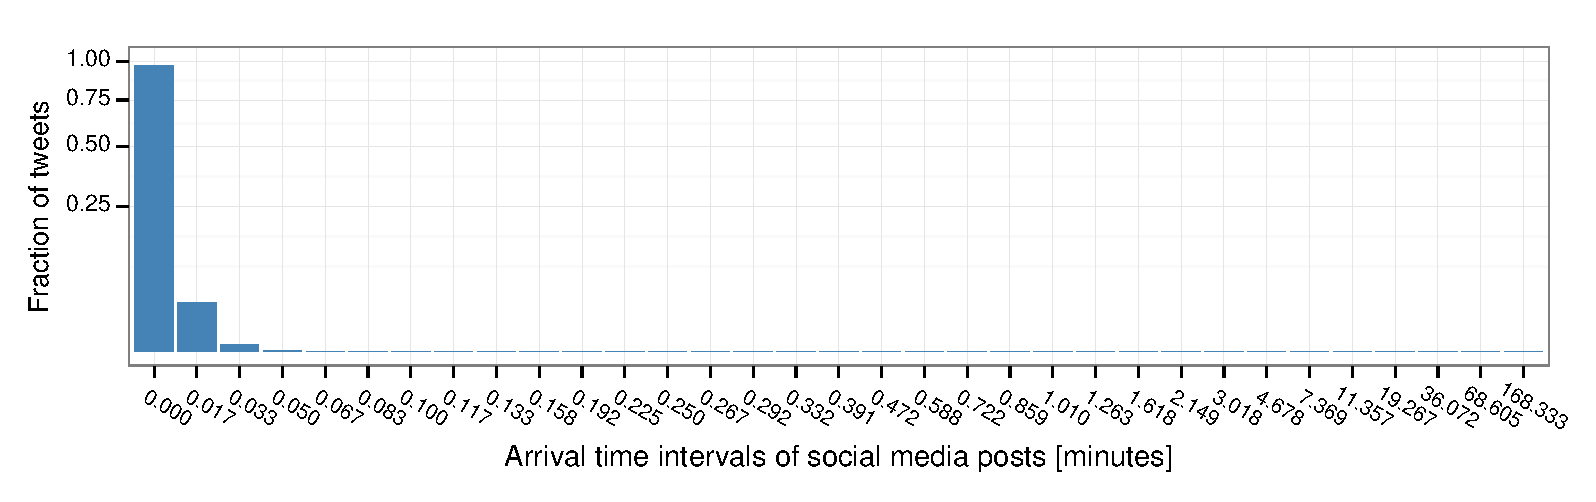
\includegraphics[width=\textwidth]{figures/nelson_mandela_buzz_example}
    \caption{User posts about the death of Nelson Mandela arrive
      almost instantly.}
    \label{fig:nelson_mandela}
  \end{subfigure}%

  ~ %add desired spacing between images, e. g. ~, \quad, \qquad, \hfill etc.
  % (or a blank line to force the subfigure onto a new line)
  \begin{subfigure}{\textwidth}
    %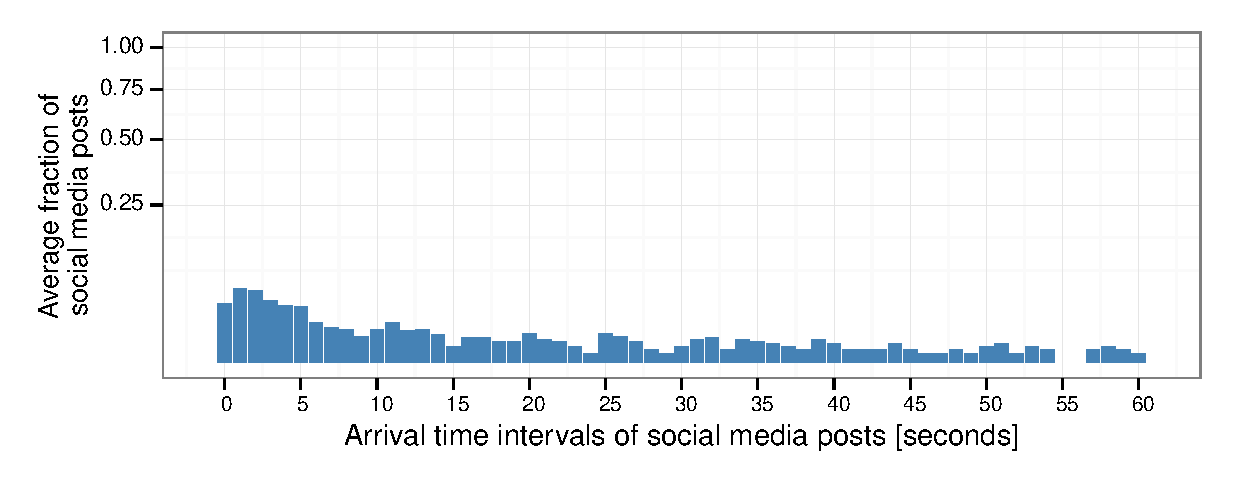
\includegraphics[width=\textwidth]{figures/may_oscar_buzz_example}
    \caption{User posts about The Oscars arriving several weeks before
      the event.}
    \label{fig:oscars}
  \end{subfigure}%
  ~ %add desired spacing between images, e. g. ~, \quad, \qquad, \hfill etc.
  % (or a blank line to force the subfigure onto a new line)

  \caption{\textbf{Illustrative examples of two events
      summarized by our method. The event [nelson, mandela] (\ref{fig:nelson_mandela}) was
      collected on 2013-12-05. Since there is a high
      concentration in the first histogram bin, we conclude that the social media posts
      for this event occur in cascades of quick successions, almost
      instantaneously. The second event, [may, oscar] (\ref{fig:oscars}) was collected
      on 2014-03-23 discussing The Oscars event that was held a few
      weeks before. The arrival times of these posts are much more spread
      out. The $y$-axis is in square root scale.} 
  }
  \label{fig:example_buzz}
\end{figure}

%\newtext{ 
We introduce a novel vectorial representation called {\em
    impact-based event model}, which models an event's impact using
  its arrival time interval distribution.  This approach is inspired
  by the {\em codebook-based representation} from the field of
  multimedia content analysis, which is used, for example, in audio
  processing and computer vision~\cite{ff,Vaizman}.  In this model, a
  \emph{codebook} of the most common time intervals between
  consecutive messages on social media about a particular event is
  learnt from a large training corpus of events.  Subsequently, each
  event is represented as a histogram where the bins are the most
  representative time intervals.  The entries of the resulting vector
  are obtained as the percentage of consecutive message pairs of the
  event that are assigned to the corresponding bin, based on their
  arrival times.  In this representation it is important to note that
  event impact is relative to an event's overall size, and that the
  model is normalized with respect to the number of messages in the
  event. Hence, the only criteria considered while deciding whether or
  not an event is high impact is the portion of messages that were
  posted close in time to each other. This denotes the urgency
  assigned to the event by the social network independently of how
  many messages were posted overall.  %}

% Experimental analysis

We study a dataset of news events gathered from news
headlines from a \emph{manually curated} list of well-known news media
accounts (e.g., @CNN, @BreakingNews, @BBCNews, etc.) in the
microblogging platform Twitter \cite{Twitter_website}
%\footnote{\url{https://twitter.com}
%  (Accessed: August 25, 2015.)} 
(a full list of all the news media
accounts is provided in the supplementary material). Headlines were
collected periodically, every hour, over the course of approximately
one year. In parallel, all the Twitter messages (called \emph{tweets})
were extracted about each news event using the public
API \cite{Twitter_API}.
%\footnote{\url{https://dev.twitter.com/} (Accessed: August 25,
%  2015.)},
% In this research, since we focus on the microblogging platform
% Twitter, we collected all the Twitter messages (called
% \emph{tweets}) produced about each news event using the publicly
% available Twitter Search API
This process was performed by automatically extracting descriptive
sets of keywords for each event using a variation of frequent itemset
extraction \cite{Tan_Steinbach_Kumar} over the event's headlines.
These sets of keywords were then used to retrieve corresponding user
tweets for each event.  Overall, the dataset contains 43,256,261
tweets that account for 5,234 events (Table~\ref{table:dataset-stats}).

We illustrate an example of an event showing the set of keywords and a
sample of tweets associated with the event
(Fig.~\ref{fig:components}).  These keywords form a semantically
meaningful event; they refer to the incident where soccer player Luis
Suarez was charged for biting another player during the FIFA World Cup
in 2014. This general collection process results in a set of social
media posts associated to an event which can encompass several memes,
viral tweets and pieces of information. Therefore, the data about an
event can be considered more complex than that of existing studies
% \cite{Castillo:2014},\cite{Szabo:2010},\cite{Lerman:2010},\cite{Tatar:2011},\cite{Pinto:2013},\cite{Ahmed:2013,
% Zaman_information_spreading},\cite{suh2010want}
\cite{Castillo:2014,Szabo:2010,Lerman:2010,Tatar:2011,Pinto:2013,Ahmed:2013,suh2010want}
which typically focus on simpler pieces of information (e.g., one
particular meme, one viral tweet etc.).  We validate the events in our
data collection process to ensure that each group of social media
posts corresponds to a meaningful news event by calculating several
clustering metrics over its social media posts. We present a detailed
description of our collection methodology and how we construct
cohesive events in the supplementary material.

\begin{table}
  \centering
  \begin{tabularx}{\textwidth}{@{}p{6cm}llll@{}}
    \toprule
    \textbf{News events' property} & \textbf{Minimum} & \textbf{Mean} & \textbf{Median} & \textbf{Maximum} \\ \midrule
    \# of posts & 1,000 & 8,254 & 2,474 & 510,920 \\
    \# of keywords & 2 & 3.77 & 3 & 39 \\
    Event duration (hours) & 0.12 & 20.93 & 7.46 & 190.43 \\ \bottomrule
  \end{tabularx}
  \caption{\bf High-level description of the dataset of news events.} \label{table:dataset-stats}
\end{table}

\begin{figure}
  %\includegraphics[width=\textwidth]{diagrams/suarez_example-crop}
  \caption{\textbf{A representative event, collected on 2014-06-25
      with keywords (left) and sample user posts (right) collected
      from the Twitter Search API. Collected user posts contain at
      least one pair of keywords. }}
  \label{fig:components}
\end{figure}


The collection of events is converted into their impact-based event
model representation. Using this model, we can identify events that
have produced similar levels of impact in the social network. In other
words, events are considered to have similar impact if the intervals
between their social media posts are similarly distributed, implying a
very much alike reaction to the events. In order to identify groups of
similar events, we perform clustering of the event models. We sort the
resulting groups of events from highest to lowest impact, according to
the concentration of social media posts in the bins that correspond to
short time intervals. We consider the events that fall in the top
cluster to be high-impact as their associated social media posts have
the shortest arrival time intervals.  In our dataset, these correspond
to roughly 8\% of the events.  We consider the next clusters in the
sorted ranking to form medium-high impact events, and so on.  Thus we
end with four groups of event histograms: high, medium-high,
medium-low and low (Fig.~\ref{fig:low_buzz_high_buzz}). This
classification of events based on their impact is independent of event
size. More details of this methodology is provided in the
supplementary material section titled `Event Model.'

\begin{figure}
  %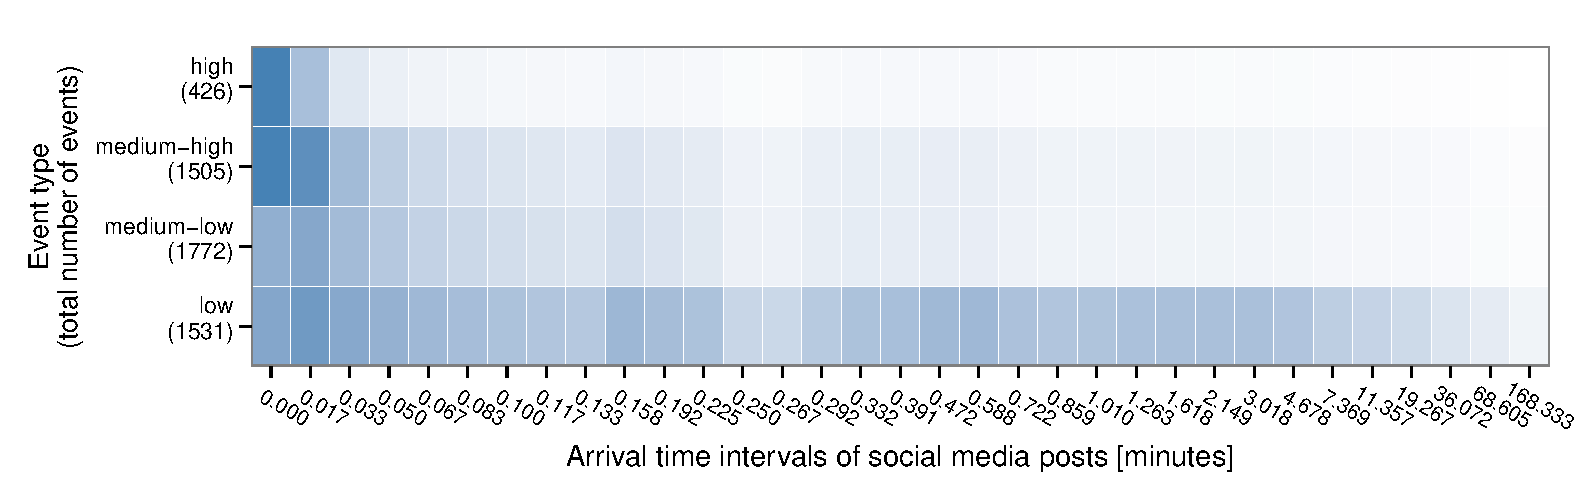
\includegraphics[width=\textwidth]{figures/heatmap_summarized}
  \caption{\textbf{Each row is the average representation of all the
      events in that clusters.  A darker cell represents a higher
      value.  The y-axis specifies the number of events in that
      cluster.  Clusters are (top to bottom): high-impact, medium-high
      medium-low and low.}
    % \inote{Mauricio: change labels of x and y-axis (to: Event type
    % (total number of events))}
  }
  \label{fig:low_buzz_high_buzz}
\end{figure}

% Results and Discussion can be combined.
\section*{Results and Discussion}
%\newtext{ 
Our main objective in this work is to analyze the
  characteristics of high-impact events which differentiate them from
  other types of events. In particular, we identify how early in an
  event's evolution is it possible to determine if an event is going
  to be of high impact in the on-line social network.

Tables~\ref{table:high-impact-sample}
and~\ref{table:low-impact-sample} show examples of events from the high-impact category and 
low-impact category. We recall that the high-impact
events are those which were in the top 8\% of the ranking obtained by
sorting the event clusters according concentration of social media
posts in bins that correspond to the shortest time interval.  Table
\ref{table:high-impact-sample}, shows two events of different sizes
(large and small) and different scopes (one global and the other more local)
categorized as high impact in our dataset. The first event, the death
of Nelson Mandela, is one of the large events in the dataset, with
$\approx$ 134,000 tweets. The histogram representation of this event,
shown in Figure \ref{fig:nelson_mandela} suggested that more than $80\%$ of
the tweets arrived almost instantaneously. This is an event of
international political and social importance, which created an
overwhelming flood of messages on social media.  Hence, it makes sense
for such an example to be placed in the high-impact category.  The
second event, on the other hand, about the 2013 Mumbai Gang Rape is of
much smaller scale, with a total of $\approx$ 1,700 tweets.  However,
this event caused considerable amount of immediate reaction on social
media, with more than $48\%$ of its messages arriving almost
instantaneously.  Despite its smaller size, and its possible
confinement to a localized on-line community, this event has been
placed in the high-impact category.

Table \ref{table:low-impact-sample} shows events that have been
classified by our methodology in the category of low impact.  The
first event, about a teen surviving after hiding in the wheel of a
airplane, had only a little more than $25\%$ of its messages arriving
instantaneously although it had over 18,000 messages.  The second
event, about the damages caused by a tornado in Canada, did not garner
much immediacy in attention since only $7\%$ of its messages arrived
instantaneously. Most of the messages of this event were spaced out in
time. Even though, we cannot say whether or not this event had
significant implications in the real-world, we can say that it did not
have considerable impact on the Twitter network. The lack of interest
could be due to several factors that are currently beyond the scope of
this work, ranging from the lack of Twitter users in the locality of
the event, to the fact that the tornado did not cause big damages.

Fig.~\ref{fig:highest}, Fig.~\ref{fig:low}, Fig.~\ref{fig:cdf-highest} and
Fig.~\ref{fig:cdf-lowest} show the average histograms and the average
cumulative distribution functions of the events corresponding to the
high and low impact categories, respectively.  Visually, the average
high-impact event vector representations starkly differs from that of
a low-impact event in that the histogram in Fig.~\ref{fig:highest}
seems to possess an exponential decay, while the histogram in
Fig.~\ref{fig:low} does not.  To test this hypothesis, we fit
exponential function of the form $f(x)=ae^{bx}$ to the event
histograms. Table~\ref{tab:curve_fitting} summarizes the results from
statistical significance tests performed on the parameters $a$ and
$b$, and on the residual least squares error used for fitting the
exponential curves.  The differences between these values is
statistically significant ($p$-value $\leq2.2\times 10^{-16}$), thus demonstrating
that high-impact events, on an average, fit the exponential decay
curve much better than their low-impact counterparts.  In addition,
Fig.~\ref{fig:param_est} shows two scatter plots with the resulting
exponential parameters $a$ and $b$.  We observe that the majority
($97.4\%$) of high-impact events have an exponent $b \leq -50$,
separating them unequivocally from other events.
%}

\input{events_example_PLOS_revision}
\begin{figure}
  \centering
  \begin{subfigure}{\textwidth}
    %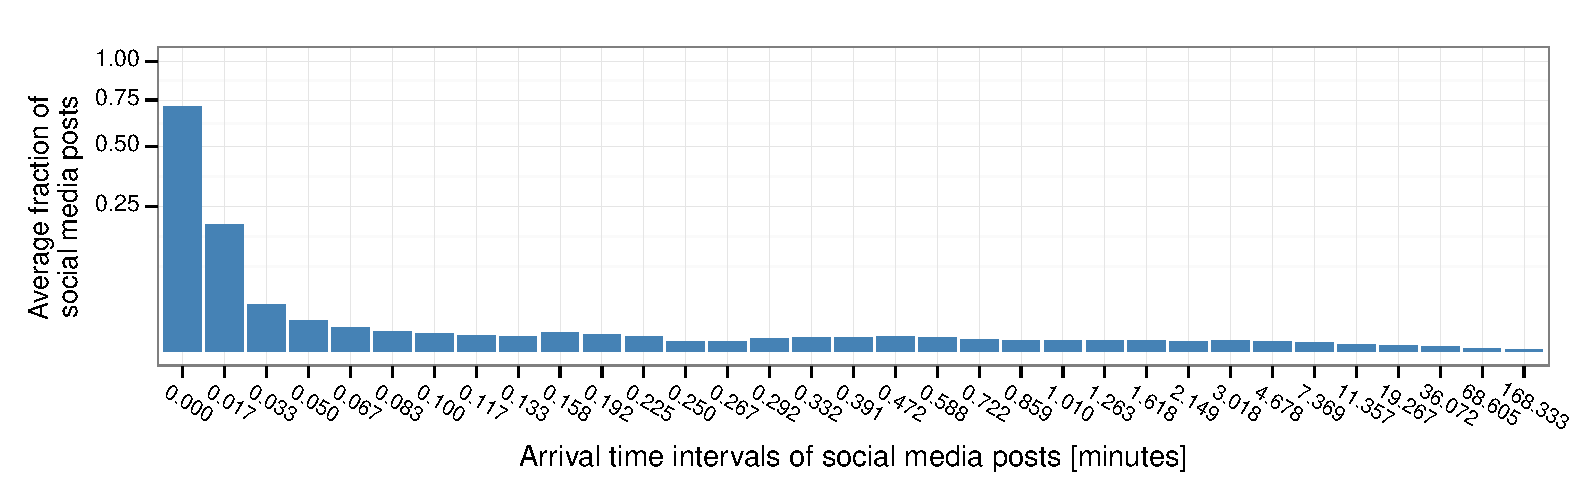
\includegraphics[width=\textwidth]{figures/avg_hist_3_7}
    \caption{High-impact event summary histogram. %\inote{Mauricio:
                                %change label for the   x-axis}
    }
    \label{fig:highest}
  \end{subfigure}%

  ~%add desired spacing between images, e. g. ~, \quad, \qquad, \hfill etc.
  % (or a blank line to force the subfigure onto a new line)
  \begin{subfigure}{\textwidth}
    %\includegraphics[width=\textwidth]{figures/avg_hist_0_1}
    \caption{Low-impact event summary histogram. %\inote{Mauricio:
                                %change label for   x-axis}
    }
    \label{fig:low}
  \end{subfigure}%
  ~ %add desired spacing between images, e. g. ~, \quad, \qquad, \hfill etc.
  % (or a blank line to force the subfigure onto a new line)

  \caption{\textbf{Fig.~\ref{fig:highest} and~\ref{fig:low} show the average
    histogram of the high-impact and lowest impact groups respectively in our dataset. The $y$-axis is in square root
      scale.
      % \inote{change labels of x and y axis}
    }}\label{fig:histograms}
\end{figure}
\begin{figure}
  \centering
  \begin{subfigure}{.5\textwidth}
    %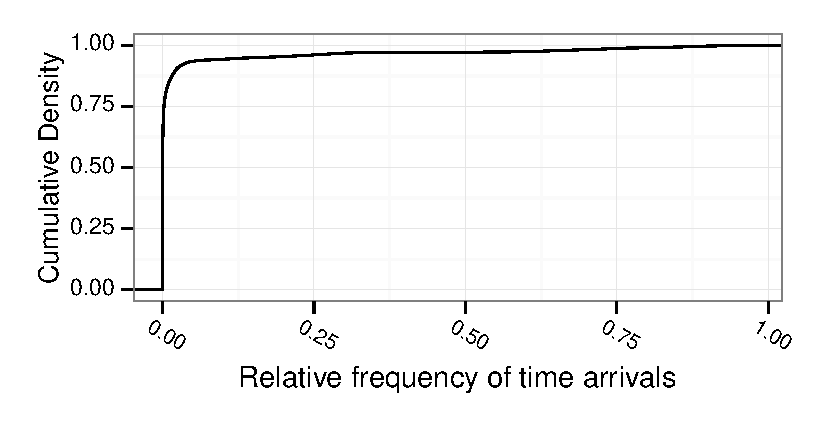
\includegraphics[width=\textwidth]{figures/cdf-highest}
    \caption{Average cumulative distribution function of high-impact events. %\inote{Mauricio:
                                %change label for the   x-axis}
    }
    \label{fig:cdf-highest}
  \end{subfigure}%
  ~%add desired spacing between images, e. g. ~, \quad, \qquad, \hfill etc.
  % (or a blank line to force the subfigure onto a new line)
  \begin{subfigure}{.5\textwidth}
    %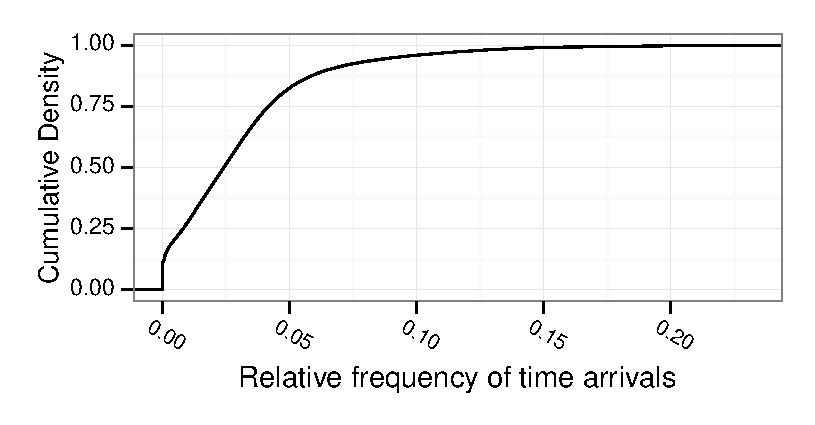
\includegraphics[width=\textwidth]{figures/cdf-lowest}
    \caption{Average cumulative distribution function of low-impact events. %\inote{Mauricio:
                                %change label for   x-axis}
    }
    \label{fig:cdf-lowest}
  \end{subfigure}%
  ~ %add desired spacing between images, e. g. ~, \quad, \qquad, \hfill etc.
  % (or a blank line to force the subfigure onto a new line)

  \caption{\textbf
      % \inote{change labels of x and y axis}
    }}\label{fig:cdfs}
\end{figure}


\begin{figure}
  \centering
  \begin{subfigure}{.5\textwidth}
    %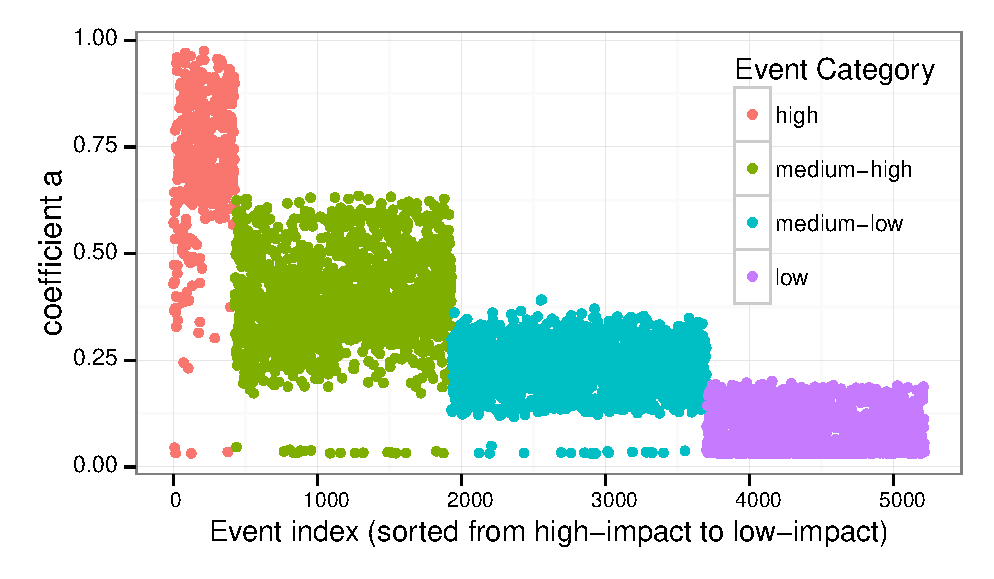
\includegraphics[width=\textwidth]{figures/param_est_a}
    \caption{Coefficient $a$ parameter estimation summary per event impact category. %\inote{Mauricio:
                                %change label for the   x-axis}
    }
    \label{fig:param-a}
  \end{subfigure}%
  ~%add desired spacing between images, e. g. ~, \quad, \qquad, \hfill etc.
  % (or a blank line to force the subfigure onto a new line)
  \begin{subfigure}{.5\textwidth}
    %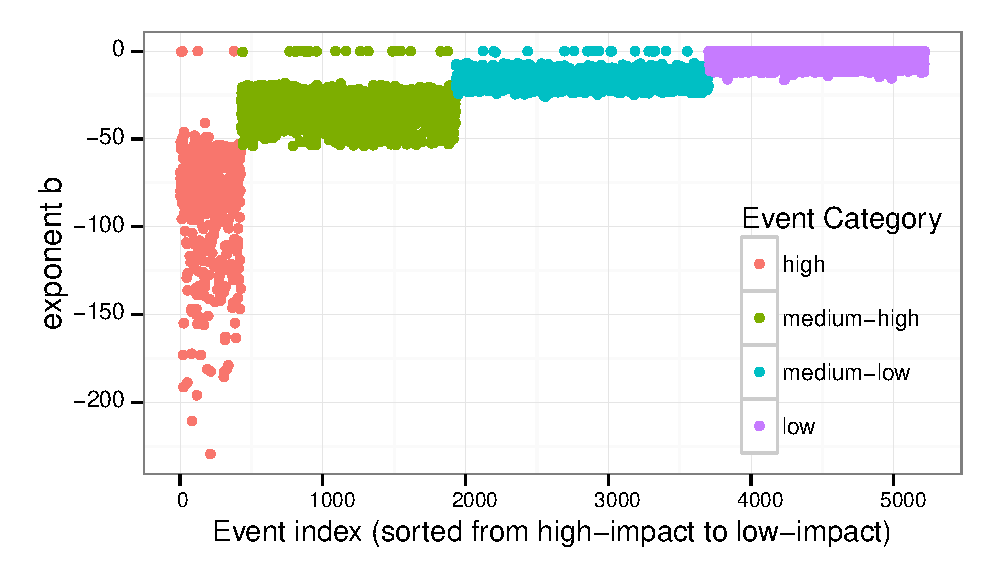
\includegraphics[width=\textwidth]{figures/param_est_b}
    \caption{Exponent $b$ parameter estimation summary per event impact category. %\inote{Mauricio:
                                %change label for   x-axis}
    }
    \label{fig:param-b}
  \end{subfigure}%
  ~ %add desired spacing between images, e. g. ~, \quad, \qquad, \hfill etc.
  % (or a blank line to force the subfigure onto a new line)

  \caption{\textbf{Fig.~\ref{fig:param-a} and~\ref{fig:param-b} show the parameter value estimation for $f(x)=ae^{bx}$.}}
  \label{fig:param_est}
\end{figure}


\begin{table}
  \centering
  \begin{tabularx}{\textwidth}{cccc}
    \toprule
    \textbf{Parameter} & \textbf{Mean (high-impact)} & \textbf{Mean (low-impact)} & \textbf{$p$-value} \\ \midrule
    $a$ & $0.7129$ & $0.0822$ & $\leq2.2\times 10^{-16}$  \\ 
    $b$ & $87.1903$ & $3.8013$ &$\leq2.2\times 10^{-16}$ \\
    Error & $0.003$ & $0.008$ & $\leq2.2\times 10^{-16}$ \\ \bottomrule
  \end{tabularx}
  \caption{\textbf
    }}
  \label{tab:curve_fitting}
\end{table}

Further analysis of the high-impact events shows significant
differences to other events, in the following aspects: (i) how the
information about these events is propagated, (ii) the characteristics
of the conversations that they generate, and (iii) how focused users
are on the news topic. In detail, high-impact events have a higher
fraction of {\em retweets} (or shares) relative to their overall
message volume. On average, a tweet from a high-impact event is
retweeted 2.36 times more than a tweet from a low impact event. The
most retweeted message in high-impact events is retweeted 7 times more
than the most retweeted message in a medium or low impact event. We
find that a small set of initial social media posts are propagated
quickly and extensively through the network without any rephrasing by
the user (plain forwarding). Intuitively, this seems justified given
general topic urgency of high-impact events. Events that are not
high-impact did not exhibit these characteristics.

Our research also revealed that high-impact events tend to spark more conversation
between users, 33.4\% more than other events. This is reflected in the
number of {\em replies} to social media posts. The number of different
users that engage in high-impact events is 32.7\% higher than in
events that are not high-impact. Posts about high-impact events are
much more topic focused than in other events. The vocabulary of unique
words as well as {\em hashtags} used in high-impact events is much
more narrow than for other events. Medium and low impact events have
over 7 times more unique hashtags than high-impact events. This is
intuitive, given that if a news item is sensational, people will
seldom deviate from the main conversation topic.

% We have presented an analysis of high-impact news events based on
% the data of their entire life-cycle in the social network. We used
% the arrival time intervals to create a model that allows us to
% classify the event according to its impact. Nevertheless,

In a real-world scenario, in order to predict if an early breaking
news story will have a considerable impact in the social network, we
will not have enough data to create its impact-based model, i.e., we
will not yet know the distribution of the speed at which the social
media posts will arrive for the event. For instance, an event can
start slowly and later produce an explosive reaction, or start
explosively and decay quickly to an overall slower message arrival
rate. Still, reliable early prediction of very high-impact news is
important in many aspects, from decisions of mass media information
coverage, to natural disaster management, brand and political image
monitoring, and so on.

For the task of early prediction of high-impact events, we use features 
that are independent of our impact-based model, such as
the retweets, the sentiment of the posts about the event, etc. 
These features are computed on the early 5\% of messages about the event.
% More details are provided in the supplementary material.
The results are an average from a 5-fold cross validation with
randomly selected 60\% training, 20\% validation and 20\% test splits.
The high-impact events are identified with a precision of 82\% using
only the earliest 5\% of the data of each event
(Table~\ref{tab:classification_results}).  Additionally, we were able to
identify with high accuracy a considerable percentage of all
high-impact events ($\approx 46\%$) at an early stage, with very few
false positives (Table~\ref{tab:classification_results} and~\ref{tab:confusion_matrix}).

\begin{table}
  %\begin{adjustwidth}{-10mm}{-10mm}
  \centering
  {\small
    \begin{tabularx}{\textwidth}{lcccc|cccc}
      \toprule
      & \multicolumn{4}{c}{\textbf{Early 5\% Tweets}} & \multicolumn{4}{c}{\textbf{All Tweets}} \\
      \midrule
      & FP-Rate & Precision & Recall & ROC-area & FP-Rate & Precision & Recall & ROC-area \\
      % \midrule
      high-impact & 0.009 & 0.819 & 0.455 & 0.900 & 0.01 & 0.830 & 0.540 & 0.945 \\
      non-high-impact & 0.545 & 0.954 & 0.991 & 0.900 &  0.460 & 0.960 & 0.990 & 0.945 \\
      \bottomrule
    \end{tabularx}
  }
  \caption{\textbf{Classification of high-impact events.}}
  \label{tab:classification_results}
  %\end{adjustwidth}
%                                                                                                                                448,1         93%
\end{table}

\begin{table}
  \centering
  % {\scriptsize
  \begin{tabularx}{\textwidth}{lcc|cc}
    \toprule
    \multirow{2}{*}{ }& \multicolumn{2}{c}{\textbf{Early 5\% Tweets}} & \multicolumn{2}{c}{\textbf{All Tweets}} \\
    \midrule
    % \cmidrule{2-5} \cline{2-5}
    & high-impact & non-high-impact & high-impact & non-high-impact \\
    % \midrule
    high-impact & $194$ & $232$ & $230$ & $196$\\
    non-high-impact & $43$ & 4,765 & 47 & 4,761 \\
    \bottomrule
  \end{tabularx}
  % }
  \caption{\textbf{Confusion matrix for high-impact events prediction.}}
  \label{tab:confusion_matrix}
\end{table}



The precision using only the early tweets is almost as good as using
all tweets in the event (0.819 to 0.830). This suggests that the
social network somehow acts as a natural filter in separating out the
high-impact events fairly early on.  The recall goes from 0.455 to
0.540. This indicates that there are some high-impact events which
require more data in order to determine what kind of impact they will
produce, or events for which impact occurs due to random conditions. A
detailed description of the features and different classification
settings are provided in the supplementary material.%\supplementary.




\section*{Conclusion}

We show that there are several properties that separate how
high-impact news events evolve in Twitter in comparison to other
events. We have created a model for events that allows us to do
unambiguous classification of high-impact events based on their impact
in the social network, in terms of the distribution of their
inter-message arrival rates. This definition does not have some of the
problems that current notions of virality and popularity have. Some
characteristics of high-impact events are that they are forwarded more
often by users, and generate a greater amount of conversation than
other events.  Social media posts from high-impact news events are
much more focused on the news topic. Our experiments show that there
are several properties that can suggest early on if an event will have
high-impact on the on-line community.  We can predict a high number of
high-impact events {\em before} the network has shown any type of
explosive reaction to them. % Using simple off-the-shelf feature based
classifiers, we can
% predict many high-impact events with high precision.
This suggests that users are collectively quick at deciding whether an
event is important or not.  However, there does exist a fraction of
events which will become high impact, despite not presenting
patterns of other high impact events during their early stages.  These
events are likely to be affected by other factors, such as random
conditions found in the social network at the moment and require
further investigation.

\section*{Supporting Information}
\subsection*{S1 Appendix}

%\section*{Acknowledgments}
%Cras egestas velit mauris, eu mollis turpis pellentesque sit amet. Interdum et malesuada fames ac ante ipsum primis in faucibus. Nam id pretium nisi. Sed ac quam id nisi malesuada congue. Sed interdum aliquet augue, at pellentesque quam rhoncus vitae.

\nolinenumbers

%\section*{References}
\bibliographystyle{plain}
\bibliography{../../report/refs}
% Either type in your references using
% \begin{thebibliography}{}
% \bibitem{}
% Text
% \end{thebibliography}
%
% OR
%
% Compile your BiBTeX database using our plos2015.bst
% style file and paste the contents of your .bbl file
% here.
% 

%\begin{thebibliography}{10}
%
%\bibitem{Ahmed:2013}
%Mohamed Ahmed, Stella Spagna, Felipe Huici, and Saverio Niccolini.
%\newblock A peek into the future: Predicting the evolution of popularity in
%  user generated content.
%\newblock In {\em Proceedings of the Sixth ACM International Conference on Web
%  Search and Data Mining}, WSDM '13, pages 607--616, New York, NY, USA, 2013.
%  ACM.
%
%\bibitem{berger2012makes}
%Jonah Berger and Katherine~L Milkman.
%\newblock What makes online content viral?
%\newblock {\em Journal of Marketing Research}, 49(2):192--205, 2012.
%
%\bibitem{Castillo:2014}
%Carlos Castillo, Mohammed El-Haddad, J\"{u}rgen Pfeffer, and Matt Stempeck.
%\newblock Characterizing the life cycle of online news stories using social
%  media reactions.
%\newblock In {\em Proceedings of the 17th ACM Conference on Computer Supported
%  Cooperative Work and Social Computing}, CSCW '14, pages 211--223, New York,
%  NY, USA, 2014. ACM.
%
%\bibitem{ff}
%L.~Fei-Fei and P.~Perona.
%\newblock A bayesian hierarchical model for learning natural scene categories.
%\newblock In {\em Computer Vision and Pattern Recognition, 2005. CVPR 2005.
%  IEEE Computer Society Conference on}, volume~2, pages 524--531 vol. 2, June
%  2005.
%
%\bibitem{gaugaz2012predicting}
%Julien Gaugaz, Patrick Siehndel, Gianluca Demartini, Tereza Iofciu, Mihai
%  Georgescu, and Nicola Henze.
%\newblock Predicting the future impact of news events.
%\newblock In {\em Advances in Information Retrieval}, pages 50--62. Springer,
%  2012.
%
%\bibitem{guerini2011exploring}
%Marco Guerini, Carlo Strapparava, and G{\"o}zde {\"O}zbal.
%\newblock Exploring text virality in social networks.
%\newblock In {\em ICWSM}, 2011.
%
%\bibitem{iribarren2011branching}
%Jos{\'e}~Luis Iribarren and Esteban Moro.
%\newblock Branching dynamics of viral information spreading.
%\newblock {\em Physical Review E}, 84(4):046116, 2011.
%
%\bibitem{Kwak:2010}
%Haewoon Kwak, Changhyun Lee, Hosung Park, and Sue Moon.
%\newblock What is twitter, a social network or a news media?
%\newblock In {\em Proceedings of the 19th International Conference on World
%  Wide Web}, WWW '10, pages 591--600, New York, NY, USA, 2010. ACM.
%
%\bibitem{Lerman:2010}
%Kristina Lerman and Tad Hogg.
%\newblock Using a model of social dynamics to predict popularity of news.
%\newblock In {\em Proceedings of the 19th International Conference on World
%  Wide Web}, WWW '10, pages 621--630, New York, NY, USA, 2010. ACM.
%
%\bibitem{mills2012virality}
%Adam~J Mills.
%\newblock Virality in social media: the spin framework.
%\newblock {\em Journal of public affairs}, 12(2):162--169, 2012.
%
%\bibitem{Pinto:2013}
%Henrique Pinto, Jussara~M. Almeida, and Marcos~A. Gon\c{c}alves.
%\newblock Using early view patterns to predict the popularity of youtube
%  videos.
%\newblock In {\em Proceedings of the Sixth ACM International Conference on Web
%  Search and Data Mining}, WSDM '13, pages 365--374, New York, NY, USA, 2013.
%  ACM.
%
%\bibitem{suh2010want}
%Bongwon Suh, Lichan Hong, Peter Pirolli, and Ed~H Chi.
%\newblock Want to be retweeted? large scale analytics on factors impacting
%  retweet in twitter network.
%\newblock In {\em Social computing (socialcom), 2010 ieee second international
%  conference on}, pages 177--184. IEEE, 2010.
%
%\bibitem{Szabo:2010}
%Gabor Szabo and Bernardo~A. Huberman.
%\newblock Predicting the popularity of online content.
%\newblock {\em Commun. ACM}, 53(8):80--88, August 2010.
%
%\bibitem{Tan_Steinbach_Kumar}
%Pang-Ning Tan, Michael Steinbach, and Vipin Kumar.
%\newblock {\em Introduction to Data Mining, (First Edition)}.
%\newblock Addison-Wesley Longman Publishing Co., Inc., Boston, MA, USA, 2005.
%
%\bibitem{Tatar:2011}
%Alexandru Tatar, J{\'e}r{\'e}mie Leguay, Panayotis Antoniadis, Arnaud Limbourg,
%  Marcelo~Dias de~Amorim, and Serge Fdida.
%\newblock Predicting the popularity of online articles based on user comments.
%\newblock In {\em Proceedings of the International Conference on Web
%  Intelligence, Mining and Semantics}, WIMS '11, pages 67:1--67:8, New York,
%  NY, USA, 2011. ACM.
%
%\bibitem{Vaizman}
%Yonatan Vaizman, Brian McFee, and Gert Lanckriet.
%\newblock Codebook-based audio feature representation for music information
%  retrieval.
%\newblock {\em IEEE/ACM Trans. Audio, Speech and Lang. Proc.},
%  22(10):1483--1493, October 2014.
%
%\bibitem{Zaman_information_spreading}
%Tauhid~R. Zaman, Ralf Herbrich, Jurgen~Van Gael, and David Stern.
%\newblock Predicting information spreading in twitter.
%
%\bibitem{ff}
%L.~Fei-Fei and P.~Perona.
%\newblock A bayesian hierarchical model for learning natural scene categories.
%\newblock In {\em Computer Vision and Pattern Recognition, 2005. CVPR 2005.
%  IEEE Computer Society Conference on}, volume~2, pages 524--531 vol. 2, June
%  2005.
%
%\bibitem{Jones72astatistical}
%Karen~Spärck Jones.
%\newblock A statistical interpretation of term specificity and its application
%  in retrieval.
%\newblock {\em Journal of Documentation}, 28:11--21, 1972.
%
%\bibitem{Tan_Steinbach_Kumar}
%Pang-Ning Tan, Michael Steinbach, and Vipin Kumar.
%\newblock {\em Introduction to Data Mining, (First Edition)}.
%\newblock Addison-Wesley Longman Publishing Co., Inc., Boston, MA, USA, 2005.
%
%
%\bibitem{Vaizman}
%Yonatan Vaizman, Brian McFee, and Gert Lanckriet.
%\newblock Codebook-based audio feature representation for music information
%  retrieval.
%\newblock {\em IEEE/ACM Trans. Audio, Speech and Lang. Proc.},
%  22(10):1483--1493, October 2014.
%
%\bibitem{Jim}
%Watch Jim Harbaugh's press conference live.
%\url{https://twitter.com/49ers/status/519202023628374016}.
%\newblock Accessed August 25, 2015..
%
%\bibitem{dallas_patient}
%Of the 48 people in context with the Dallas patient, no one is showing any symptoms.
%\url{https://twitter.com/PzFeed/status/519203692898435072}.
%\newblock Accessed August 25, 2015.
%
%\bibitem{nelson_mandela_dead}
%Death of Nelson Mandela.
%\url{https://en.wikipedia.org/wiki/Death_of_Nelson_Mandela}.
%\newblock Accessed August 25, 2015.
%
%\bibitem{chile_elections}
%Chile elections.
%\url{http://www.telegraph.co.uk/news/worldnews/southamerica/chile/10188216/Chilean-presidential-candidate-pulls-out-of-election-with-depression.html}/
%\newblock Accessed August 25, 2015.
%
%\bibitem{Twitter_website}
%Twitter.
%\url{https://twitter.com}.
%\newblock Accessed August 25, 2015.
%
%\bibitem{Twitter_API}
%Twitter API.
%\url{https://dev.twitter.com/}.
%\newblock Accessed August 25, 2015.
%
%\end{thebibliography}
%
%
%

\end{document}

